Development of DRB started with development in phases which focus on particular need of project.
Various phases and their detail are given below -:
\begin{itemize}
\item Phase I : \\
	During Phase I, we wrote code in JavaScript to compute all the required output variable.
We use different controllers for the application. Controller named BeamControl fetch the data from the user and perform operations and gives out required result.
\item Phase II (\LaTeX{}) : \\
	During Phase II, we wrote code in JavaScript to compute all the required output variable.
We use different controllers for the application. Controller named BeamControl fetch the data from the user and perform operations and gives out required result.
	
\item Phase III : \\
	During phase III, we provided web interface to this software using Django. Djanog was used
	to get input from user and write input.sage file for particular user then civil.sh 
	is called by passing name of user directory to it and then get output PDF.
\item Phase IV : \\
	During phase IV, we improved the code structure and added additional 
	functionality like sending PDF as email and accepting input as CSV file.
	Finally, the UI was improved and made responsive.
\item Phase V : \\
During phase V, we tested the software for various conditions and then applied required error control and messaging 
mechanism. initialfile.py file was created to save software from problem of server restart which can causes processing user request to stop. so, that 
the interrupted request of user can be restart and send PDF.
\item Phase VI-: \\ 
During final phase, we documented the project( developers documentation and README.md) using doxygen and wrote the report for this software.    
\end{itemize}     

\begin{figure}[H] 
\centering 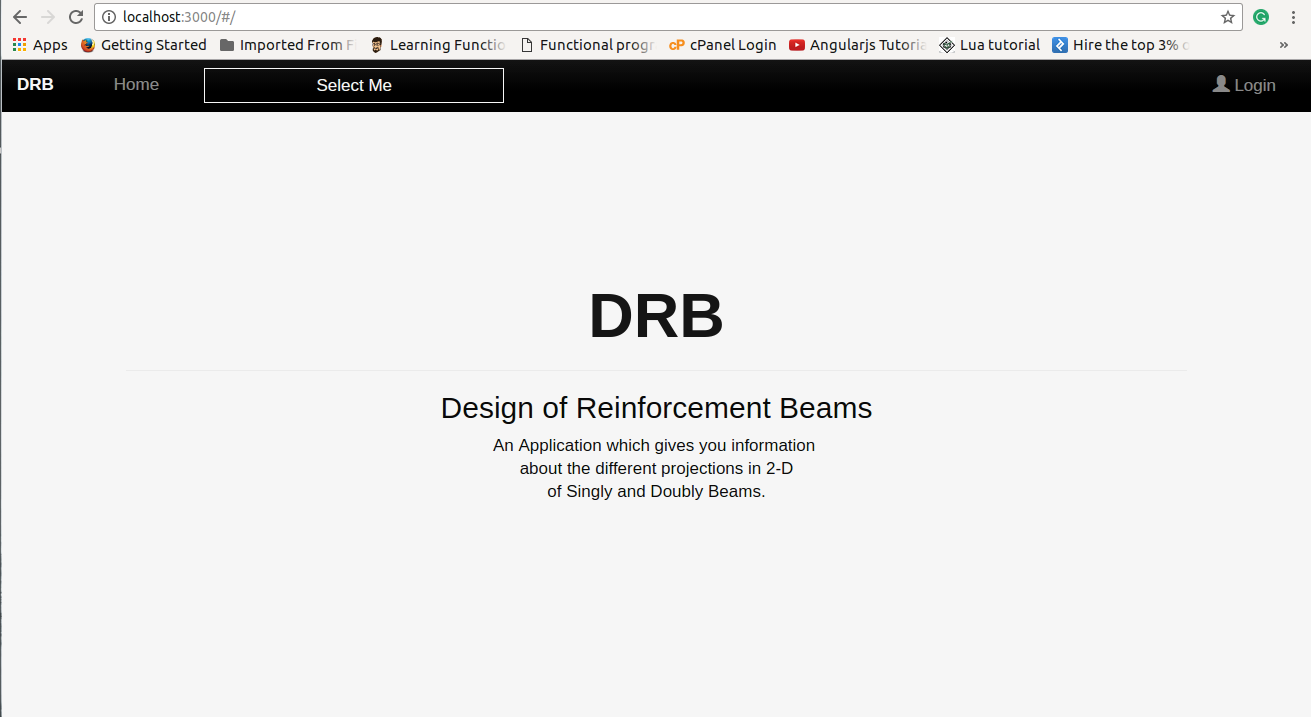
\includegraphics[scale=0.32]{images/output/screen1.png}
\caption{Home page of DRB}
\label{fig:1}
\end{figure}
This is the first interface that is shown to the user. This is the Home page.
It brings a nice UI to get input from user about the Number of storeys and 
some factor affecting the structure. It also provides the user some 
additional features as an aid like moving to specific operations the user want to do. There is an icon of logo i.e DRB which directs the user to home. There is also an login icon for user to login from different clients like gmail and facebook.\ref{fig:1}
\begin{figure}[H] 
\centering 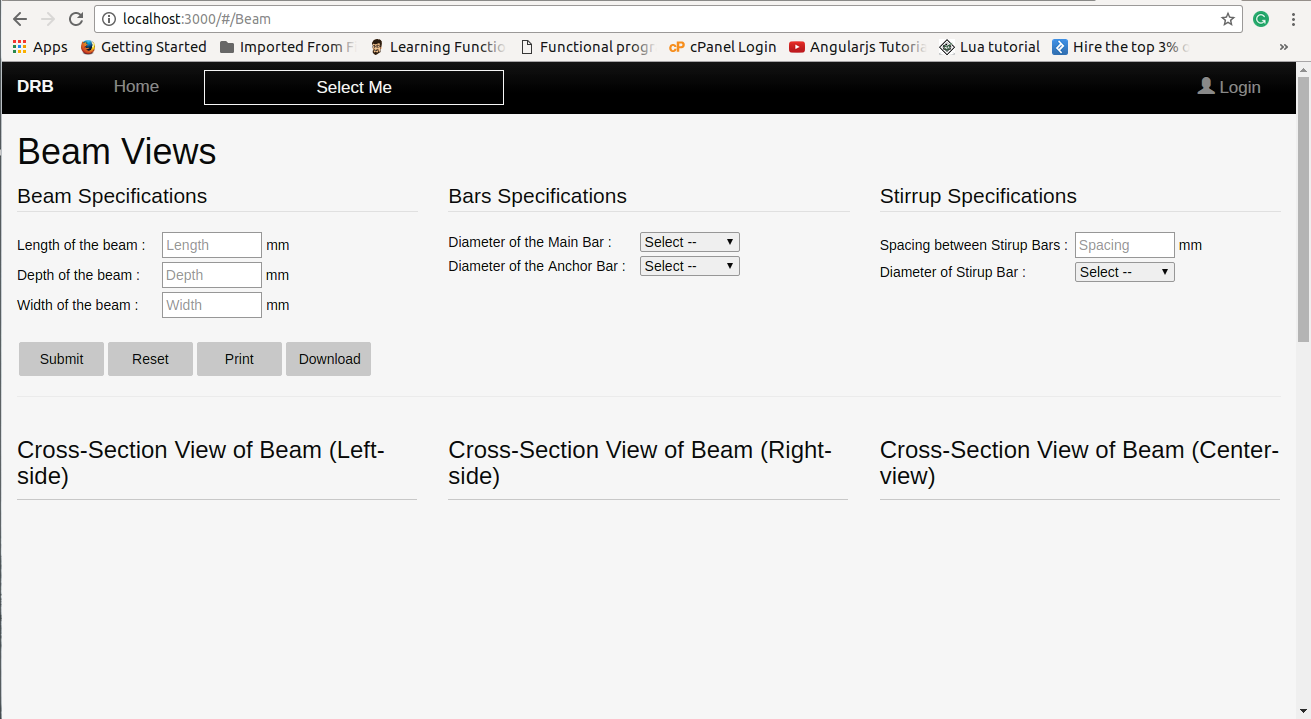
\includegraphics[scale=0.32]{images/output/screen2.png}
\caption{Beam Views}
\label{fig:2}
\end{figure}  


After filling the required data click the 'Submit' button on the page, Different views are drawn under the specific places.\ref{fig:2}

\begin{figure}[H] 
\centering 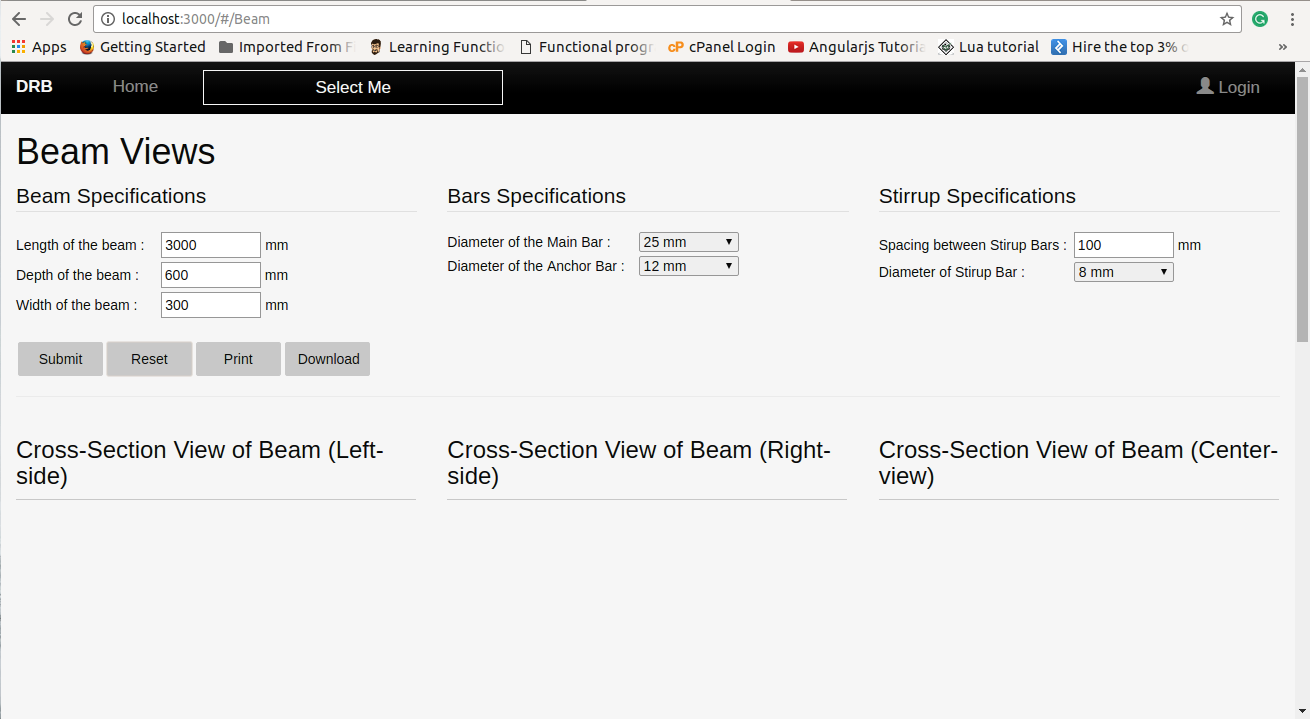
\includegraphics[scale=0.32]{images/output/screen3.png}
\caption{filling values}
\label{fig:3}
\end{figure}

After filling certain values.\ref{fig:3}

\begin{figure}[H] 
\centering 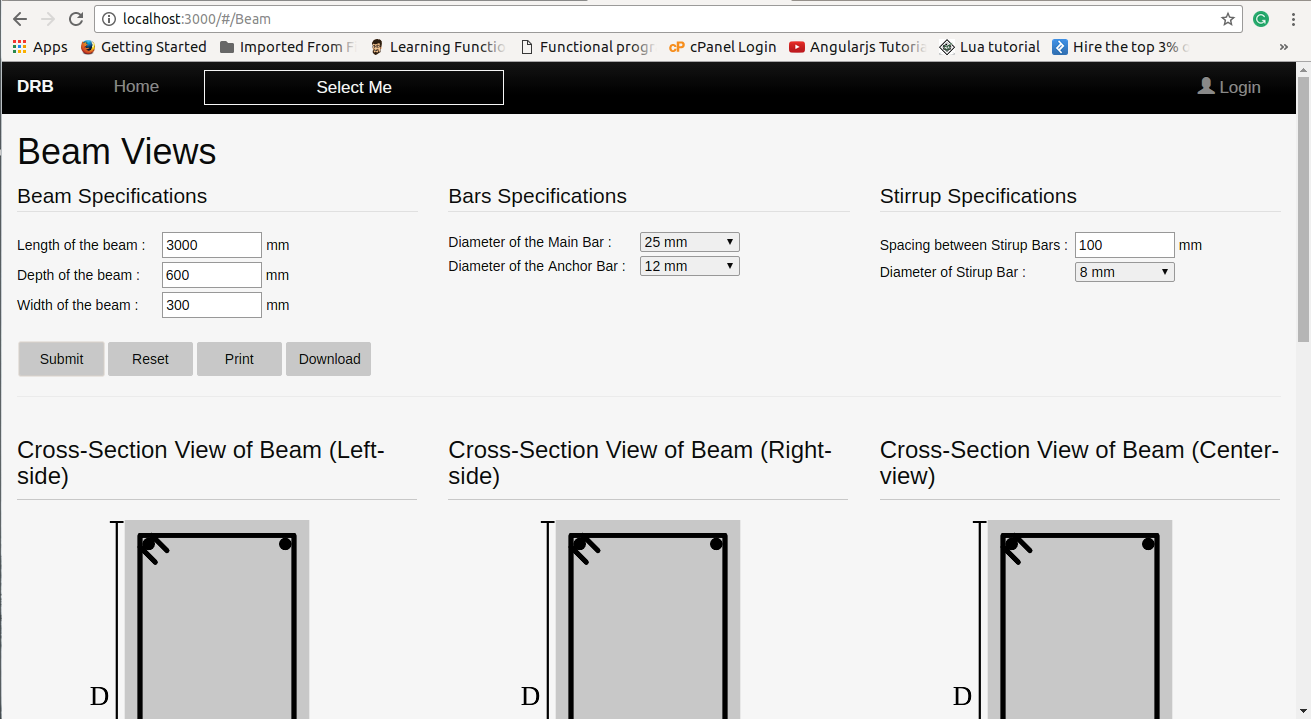
\includegraphics[scale=0.31]{images/output/screen4.png}
\caption{resulting view}
\label{fig:4}
\end{figure}

\begin{figure}[H] 
\centering 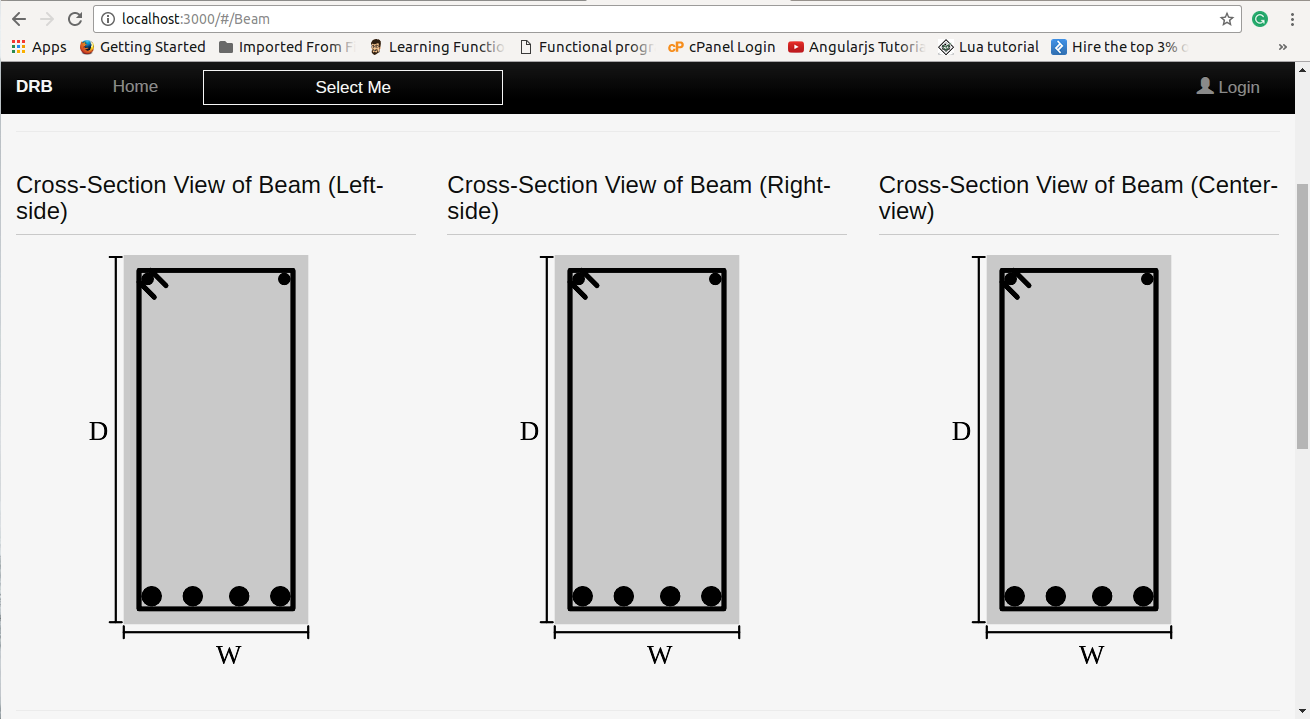
\includegraphics[scale=0.31]{images/output/screen5.png}
\caption{resulting view}
\label{fig:5}
\end{figure}

Output of the result Cross section view of beam(left, right and center)\ref{fig:4}\ref{fig:5}

\begin{figure}[H] 
\centering 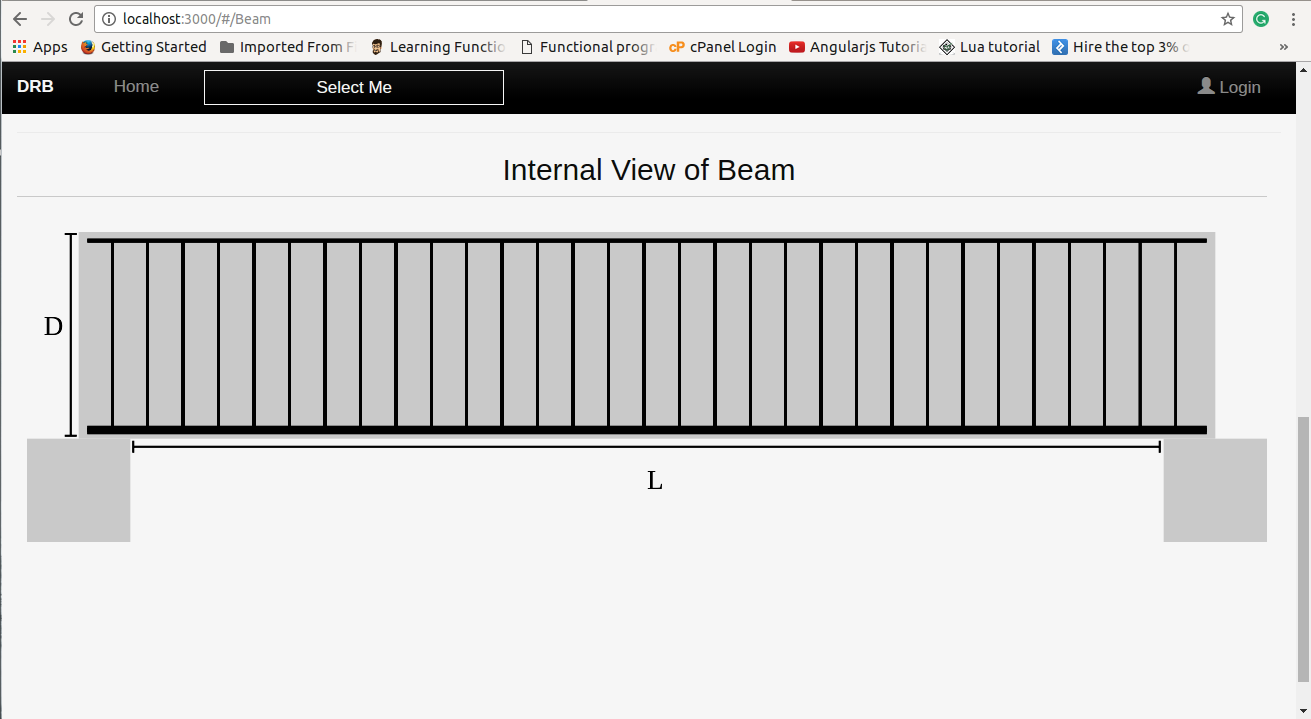
\includegraphics[scale=0.31]{images/output/screen6.png}
\caption{resulting view}
\label{fig:6}
\end{figure}

Output of the Internal view of the beam.\ref{fig:6}

\begin{figure}[H] 
\centering 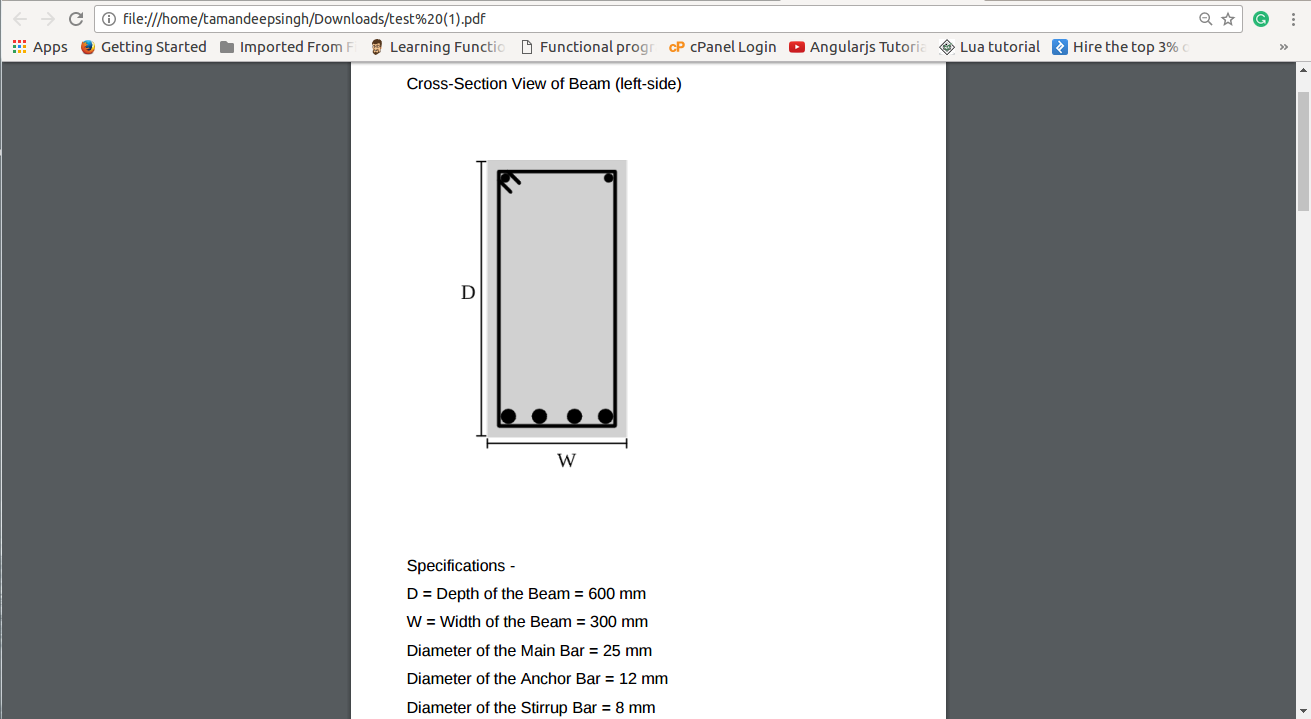
\includegraphics[scale=0.31]{images/output/screen7.png}
\caption{Result in pdf format and other information}
\label{fig:7}
\end{figure}

Output View of cross section of beam (Left side)\ref{fig:7}.

\begin{figure}[H] 
\centering 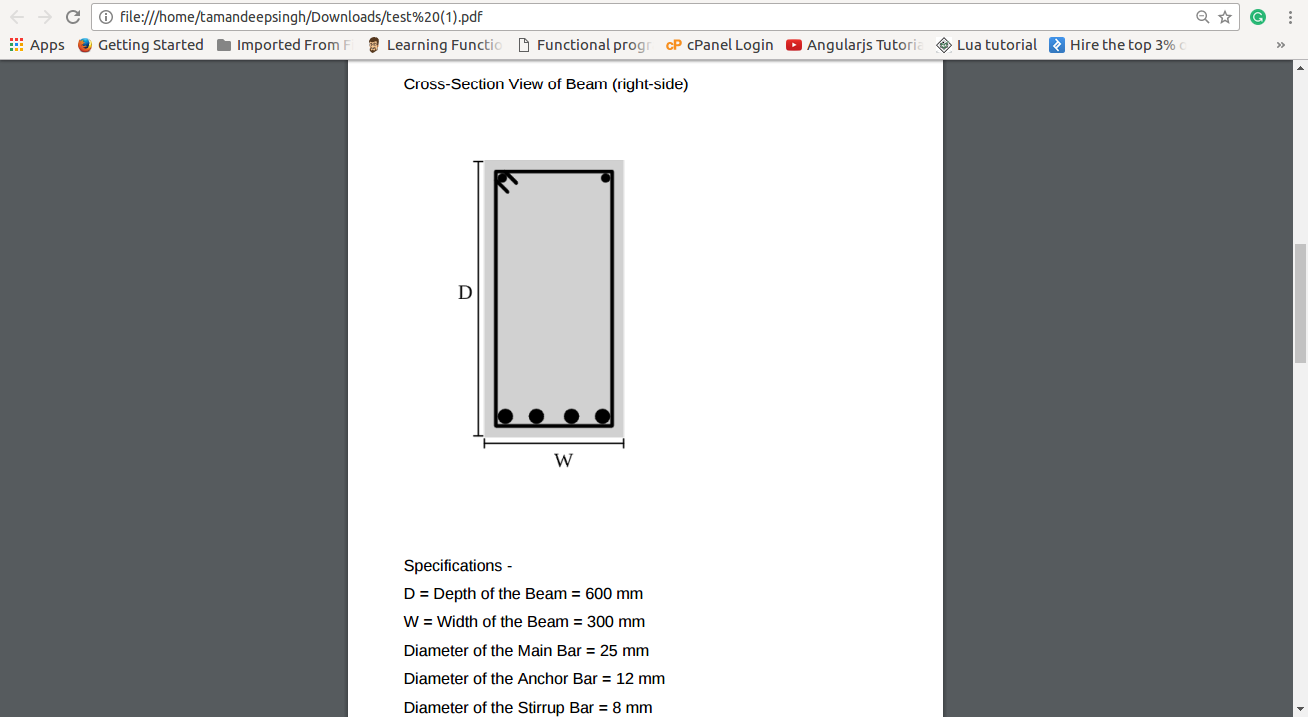
\includegraphics[scale=0.31]{images/output/screen8.png}
\caption{Result in pdf format and other information}
\label{fig:8}
\end{figure}

Output View of cross section of beam (Right side) \ref{fig:8}.

\begin{figure}[H] 
\centering 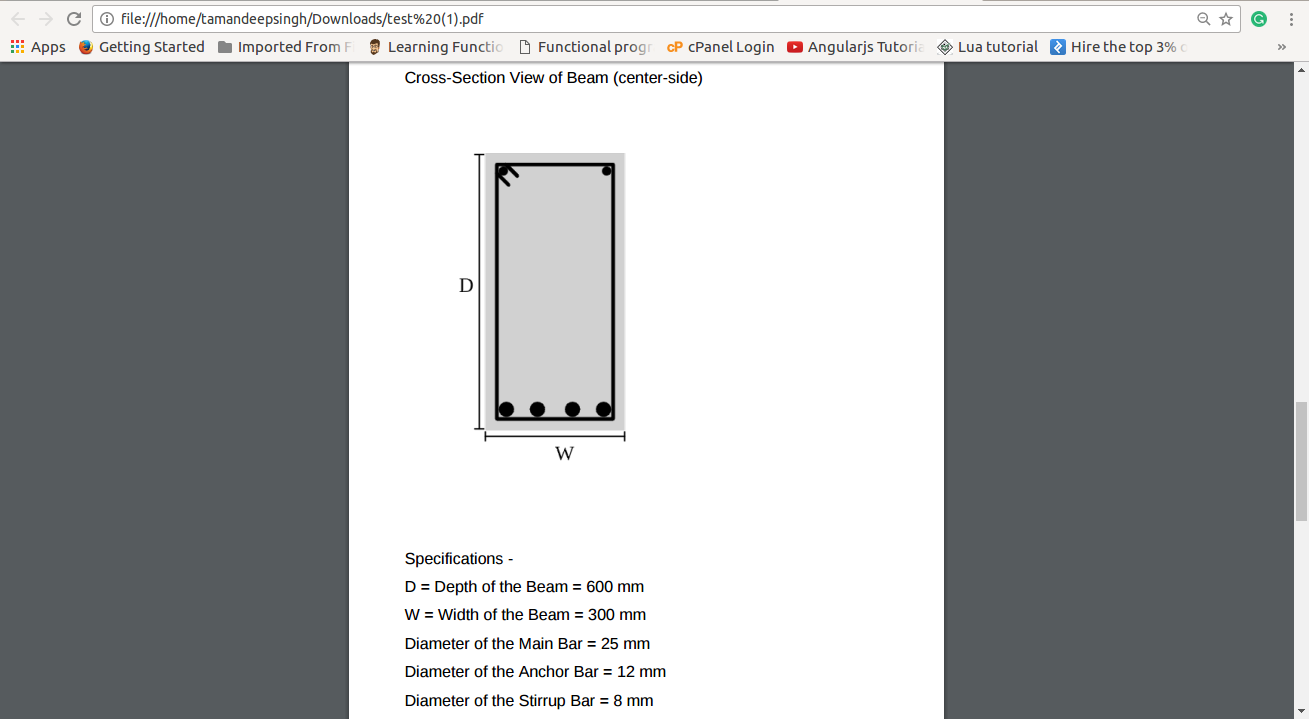
\includegraphics[scale=0.31]{images/output/screen9.png}
\caption{Result in pdf format and other information}
\label{fig:9}
\end{figure}

Output View of cross section of beam (Center side)\ref{fig:9}.

\begin{figure}[H] 
\centering 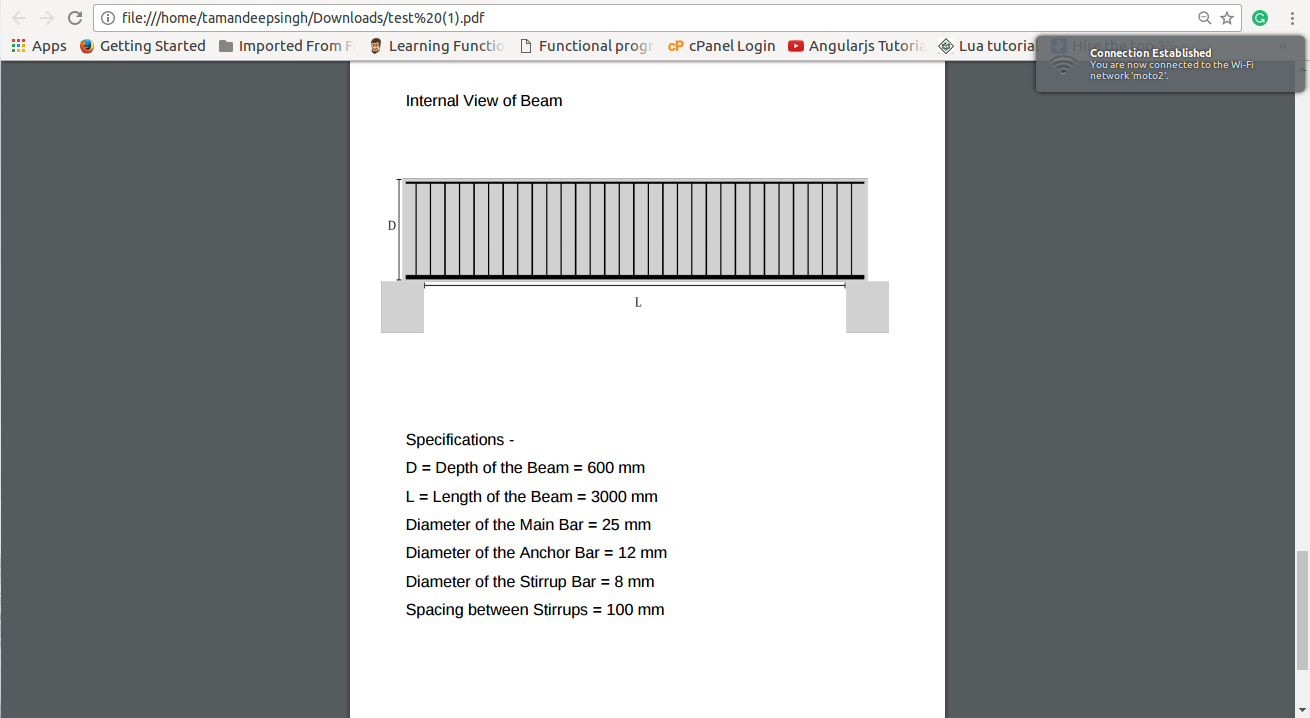
\includegraphics[scale=0.31]{images/output/screen10.png}
\caption{Result in pdf format and other information}
\label{fig:10}
\end{figure}

Output View of Internal view of the Beam\ref{fig:10}.
